\PassOptionsToPackage{unicode=true}{hyperref} % options for packages loaded elsewhere
\PassOptionsToPackage{hyphens}{url}
%
\documentclass[]{article}
\usepackage{lmodern}
\usepackage{amssymb,amsmath}
\usepackage{ifxetex,ifluatex}
\usepackage{fixltx2e} % provides \textsubscript
\ifnum 0\ifxetex 1\fi\ifluatex 1\fi=0 % if pdftex
  \usepackage[T1]{fontenc}
  \usepackage[utf8]{inputenc}
  \usepackage{textcomp} % provides euro and other symbols
\else % if luatex or xelatex
  \usepackage{unicode-math}
  \defaultfontfeatures{Ligatures=TeX,Scale=MatchLowercase}
\fi
% use upquote if available, for straight quotes in verbatim environments
\IfFileExists{upquote.sty}{\usepackage{upquote}}{}
% use microtype if available
\IfFileExists{microtype.sty}{%
\usepackage[]{microtype}
\UseMicrotypeSet[protrusion]{basicmath} % disable protrusion for tt fonts
}{}
\IfFileExists{parskip.sty}{%
\usepackage{parskip}
}{% else
\setlength{\parindent}{0pt}
\setlength{\parskip}{6pt plus 2pt minus 1pt}
}
\usepackage{hyperref}
\hypersetup{
            pdftitle={Association Rule Mining},
            pdfauthor={Mehmet Ali Akyol},
            pdfborder={0 0 0},
            breaklinks=true}
\urlstyle{same}  % don't use monospace font for urls
\usepackage[margin=1in]{geometry}
\usepackage{color}
\usepackage{fancyvrb}
\newcommand{\VerbBar}{|}
\newcommand{\VERB}{\Verb[commandchars=\\\{\}]}
\DefineVerbatimEnvironment{Highlighting}{Verbatim}{commandchars=\\\{\}}
% Add ',fontsize=\small' for more characters per line
\usepackage{framed}
\definecolor{shadecolor}{RGB}{248,248,248}
\newenvironment{Shaded}{\begin{snugshade}}{\end{snugshade}}
\newcommand{\AlertTok}[1]{\textcolor[rgb]{0.94,0.16,0.16}{#1}}
\newcommand{\AnnotationTok}[1]{\textcolor[rgb]{0.56,0.35,0.01}{\textbf{\textit{#1}}}}
\newcommand{\AttributeTok}[1]{\textcolor[rgb]{0.77,0.63,0.00}{#1}}
\newcommand{\BaseNTok}[1]{\textcolor[rgb]{0.00,0.00,0.81}{#1}}
\newcommand{\BuiltInTok}[1]{#1}
\newcommand{\CharTok}[1]{\textcolor[rgb]{0.31,0.60,0.02}{#1}}
\newcommand{\CommentTok}[1]{\textcolor[rgb]{0.56,0.35,0.01}{\textit{#1}}}
\newcommand{\CommentVarTok}[1]{\textcolor[rgb]{0.56,0.35,0.01}{\textbf{\textit{#1}}}}
\newcommand{\ConstantTok}[1]{\textcolor[rgb]{0.00,0.00,0.00}{#1}}
\newcommand{\ControlFlowTok}[1]{\textcolor[rgb]{0.13,0.29,0.53}{\textbf{#1}}}
\newcommand{\DataTypeTok}[1]{\textcolor[rgb]{0.13,0.29,0.53}{#1}}
\newcommand{\DecValTok}[1]{\textcolor[rgb]{0.00,0.00,0.81}{#1}}
\newcommand{\DocumentationTok}[1]{\textcolor[rgb]{0.56,0.35,0.01}{\textbf{\textit{#1}}}}
\newcommand{\ErrorTok}[1]{\textcolor[rgb]{0.64,0.00,0.00}{\textbf{#1}}}
\newcommand{\ExtensionTok}[1]{#1}
\newcommand{\FloatTok}[1]{\textcolor[rgb]{0.00,0.00,0.81}{#1}}
\newcommand{\FunctionTok}[1]{\textcolor[rgb]{0.00,0.00,0.00}{#1}}
\newcommand{\ImportTok}[1]{#1}
\newcommand{\InformationTok}[1]{\textcolor[rgb]{0.56,0.35,0.01}{\textbf{\textit{#1}}}}
\newcommand{\KeywordTok}[1]{\textcolor[rgb]{0.13,0.29,0.53}{\textbf{#1}}}
\newcommand{\NormalTok}[1]{#1}
\newcommand{\OperatorTok}[1]{\textcolor[rgb]{0.81,0.36,0.00}{\textbf{#1}}}
\newcommand{\OtherTok}[1]{\textcolor[rgb]{0.56,0.35,0.01}{#1}}
\newcommand{\PreprocessorTok}[1]{\textcolor[rgb]{0.56,0.35,0.01}{\textit{#1}}}
\newcommand{\RegionMarkerTok}[1]{#1}
\newcommand{\SpecialCharTok}[1]{\textcolor[rgb]{0.00,0.00,0.00}{#1}}
\newcommand{\SpecialStringTok}[1]{\textcolor[rgb]{0.31,0.60,0.02}{#1}}
\newcommand{\StringTok}[1]{\textcolor[rgb]{0.31,0.60,0.02}{#1}}
\newcommand{\VariableTok}[1]{\textcolor[rgb]{0.00,0.00,0.00}{#1}}
\newcommand{\VerbatimStringTok}[1]{\textcolor[rgb]{0.31,0.60,0.02}{#1}}
\newcommand{\WarningTok}[1]{\textcolor[rgb]{0.56,0.35,0.01}{\textbf{\textit{#1}}}}
\usepackage{graphicx,grffile}
\makeatletter
\def\maxwidth{\ifdim\Gin@nat@width>\linewidth\linewidth\else\Gin@nat@width\fi}
\def\maxheight{\ifdim\Gin@nat@height>\textheight\textheight\else\Gin@nat@height\fi}
\makeatother
% Scale images if necessary, so that they will not overflow the page
% margins by default, and it is still possible to overwrite the defaults
% using explicit options in \includegraphics[width, height, ...]{}
\setkeys{Gin}{width=\maxwidth,height=\maxheight,keepaspectratio}
\setlength{\emergencystretch}{3em}  % prevent overfull lines
\providecommand{\tightlist}{%
  \setlength{\itemsep}{0pt}\setlength{\parskip}{0pt}}
\setcounter{secnumdepth}{0}
% Redefines (sub)paragraphs to behave more like sections
\ifx\paragraph\undefined\else
\let\oldparagraph\paragraph
\renewcommand{\paragraph}[1]{\oldparagraph{#1}\mbox{}}
\fi
\ifx\subparagraph\undefined\else
\let\oldsubparagraph\subparagraph
\renewcommand{\subparagraph}[1]{\oldsubparagraph{#1}\mbox{}}
\fi

% set default figure placement to htbp
\makeatletter
\def\fps@figure{htbp}
\makeatother


\title{Association Rule Mining}
\author{Mehmet Ali Akyol}
\date{2/10/2020}

\begin{document}
\maketitle

The objective of this document is to give a brief introduction to
association mining. This document assumes the users have no prior
knowledge of R. After completing this tutorial, you will be able to:

\begin{itemize}
\tightlist
\item
  Mine associated sets
\item
  Find closed and maximal item sets
\item
  Use different interestingness measures
\item
  Visualize associations
\end{itemize}

Let's load our main data to use:

\begin{Shaded}
\begin{Highlighting}[]
\KeywordTok{load}\NormalTok{(}\KeywordTok{url}\NormalTok{(}\StringTok{"http://www.rdatamining.com/data/titanic.raw.rdata?attredirects=0&d=1"}\NormalTok{))}
\end{Highlighting}
\end{Shaded}

Install and load packages:

\begin{Shaded}
\begin{Highlighting}[]
\CommentTok{#install.packages("arules")}
\KeywordTok{require}\NormalTok{(arules)}
\end{Highlighting}
\end{Shaded}

\hypertarget{maximal-and-closed-itemsets}{%
\subsubsection{Maximal and Closed
Itemsets}\label{maximal-and-closed-itemsets}}

Mine the closed and maximal itemsets:

\begin{Shaded}
\begin{Highlighting}[]
\NormalTok{closed.itemset <-}\StringTok{ }\KeywordTok{apriori}\NormalTok{(titanic.raw, }\DataTypeTok{parameter =} \KeywordTok{list}\NormalTok{(}\DataTypeTok{target=}\StringTok{"closed frequent itemsets"}\NormalTok{))}
\end{Highlighting}
\end{Shaded}

\begin{verbatim}
## Apriori
## 
## Parameter specification:
##  confidence minval smax arem  aval originalSupport maxtime support minlen maxlen                   target
##          NA    0.1    1 none FALSE            TRUE       5     0.1      1     10 closed frequent itemsets
##    ext
##  FALSE
## 
## Algorithmic control:
##  filter tree heap memopt load sort verbose
##     0.1 TRUE TRUE  FALSE TRUE    2    TRUE
## 
## Absolute minimum support count: 220 
## 
## set item appearances ...[0 item(s)] done [0.00s].
## set transactions ...[10 item(s), 2201 transaction(s)] done [0.00s].
## sorting and recoding items ... [9 item(s)] done [0.00s].
## creating transaction tree ... done [0.00s].
## checking subsets of size 1 2 3 4 done [0.00s].
## filtering closed item sets ... done [0.00s].
## writing ... [31 set(s)] done [0.00s].
## creating S4 object  ... done [0.00s].
\end{verbatim}

\begin{Shaded}
\begin{Highlighting}[]
\NormalTok{max.itemset <-}\StringTok{ }\KeywordTok{apriori}\NormalTok{(titanic.raw, }\DataTypeTok{parameter =} \KeywordTok{list}\NormalTok{(}\DataTypeTok{target=}\StringTok{"maximally frequent itemsets"}\NormalTok{))}
\end{Highlighting}
\end{Shaded}

\begin{verbatim}
## Apriori
## 
## Parameter specification:
##  confidence minval smax arem  aval originalSupport maxtime support minlen maxlen
##          NA    0.1    1 none FALSE            TRUE       5     0.1      1     10
##                       target   ext
##  maximally frequent itemsets FALSE
## 
## Algorithmic control:
##  filter tree heap memopt load sort verbose
##     0.1 TRUE TRUE  FALSE TRUE    2    TRUE
## 
## Absolute minimum support count: 220 
## 
## set item appearances ...[0 item(s)] done [0.00s].
## set transactions ...[10 item(s), 2201 transaction(s)] done [0.00s].
## sorting and recoding items ... [9 item(s)] done [0.00s].
## creating transaction tree ... done [0.00s].
## checking subsets of size 1 2 3 4 done [0.00s].
## filtering maximal item sets ... done [0.00s].
## writing ... [6 set(s)] done [0.00s].
## creating S4 object  ... done [0.00s].
\end{verbatim}

\hypertarget{initial-mining}{%
\subsubsection{Initial Mining}\label{initial-mining}}

Mine initial association rules with default settings (i.e
\texttt{minsup\ =\ 0.1}, \texttt{mincon\ =\ 0.8},
\texttt{maxlength\ =\ 10}).

\begin{Shaded}
\begin{Highlighting}[]
\NormalTok{rules <-}\StringTok{ }\KeywordTok{apriori}\NormalTok{(titanic.raw)}
\end{Highlighting}
\end{Shaded}

\begin{verbatim}
## Apriori
## 
## Parameter specification:
##  confidence minval smax arem  aval originalSupport maxtime support minlen maxlen target   ext
##         0.8    0.1    1 none FALSE            TRUE       5     0.1      1     10  rules FALSE
## 
## Algorithmic control:
##  filter tree heap memopt load sort verbose
##     0.1 TRUE TRUE  FALSE TRUE    2    TRUE
## 
## Absolute minimum support count: 220 
## 
## set item appearances ...[0 item(s)] done [0.00s].
## set transactions ...[10 item(s), 2201 transaction(s)] done [0.00s].
## sorting and recoding items ... [9 item(s)] done [0.00s].
## creating transaction tree ... done [0.00s].
## checking subsets of size 1 2 3 4 done [0.00s].
## writing ... [27 rule(s)] done [0.00s].
## creating S4 object  ... done [0.00s].
\end{verbatim}

This creates a total of 27 rules, which is not a lot. However when you
have a larger dataset, you are likely to get a much bigger rule set.

Let's inspect the rules:

\begin{Shaded}
\begin{Highlighting}[]
\KeywordTok{inspect}\NormalTok{(rules)}
\end{Highlighting}
\end{Shaded}

\begin{verbatim}
##      lhs                                   rhs           support   confidence lift      count
## [1]  {}                                 => {Age=Adult}   0.9504771 0.9504771  1.0000000 2092 
## [2]  {Class=2nd}                        => {Age=Adult}   0.1185825 0.9157895  0.9635051  261 
## [3]  {Class=1st}                        => {Age=Adult}   0.1449341 0.9815385  1.0326798  319 
## [4]  {Sex=Female}                       => {Age=Adult}   0.1930940 0.9042553  0.9513700  425 
## [5]  {Class=3rd}                        => {Age=Adult}   0.2848705 0.8881020  0.9343750  627 
## [6]  {Survived=Yes}                     => {Age=Adult}   0.2971377 0.9198312  0.9677574  654 
## [7]  {Class=Crew}                       => {Sex=Male}    0.3916402 0.9740113  1.2384742  862 
## [8]  {Class=Crew}                       => {Age=Adult}   0.4020900 1.0000000  1.0521033  885 
## [9]  {Survived=No}                      => {Sex=Male}    0.6197183 0.9154362  1.1639949 1364 
## [10] {Survived=No}                      => {Age=Adult}   0.6533394 0.9651007  1.0153856 1438 
## [11] {Sex=Male}                         => {Age=Adult}   0.7573830 0.9630272  1.0132040 1667 
## [12] {Sex=Female,Survived=Yes}          => {Age=Adult}   0.1435711 0.9186047  0.9664669  316 
## [13] {Class=3rd,Sex=Male}               => {Survived=No} 0.1917310 0.8274510  1.2222950  422 
## [14] {Class=3rd,Survived=No}            => {Age=Adult}   0.2162653 0.9015152  0.9484870  476 
## [15] {Class=3rd,Sex=Male}               => {Age=Adult}   0.2099046 0.9058824  0.9530818  462 
## [16] {Sex=Male,Survived=Yes}            => {Age=Adult}   0.1535666 0.9209809  0.9689670  338 
## [17] {Class=Crew,Survived=No}           => {Sex=Male}    0.3044071 0.9955423  1.2658514  670 
## [18] {Class=Crew,Survived=No}           => {Age=Adult}   0.3057701 1.0000000  1.0521033  673 
## [19] {Class=Crew,Sex=Male}              => {Age=Adult}   0.3916402 1.0000000  1.0521033  862 
## [20] {Class=Crew,Age=Adult}             => {Sex=Male}    0.3916402 0.9740113  1.2384742  862 
## [21] {Sex=Male,Survived=No}             => {Age=Adult}   0.6038164 0.9743402  1.0251065 1329 
## [22] {Age=Adult,Survived=No}            => {Sex=Male}    0.6038164 0.9242003  1.1751385 1329 
## [23] {Class=3rd,Sex=Male,Survived=No}   => {Age=Adult}   0.1758292 0.9170616  0.9648435  387 
## [24] {Class=3rd,Age=Adult,Survived=No}  => {Sex=Male}    0.1758292 0.8130252  1.0337773  387 
## [25] {Class=3rd,Sex=Male,Age=Adult}     => {Survived=No} 0.1758292 0.8376623  1.2373791  387 
## [26] {Class=Crew,Sex=Male,Survived=No}  => {Age=Adult}   0.3044071 1.0000000  1.0521033  670 
## [27] {Class=Crew,Age=Adult,Survived=No} => {Sex=Male}    0.3044071 0.9955423  1.2658514  670
\end{verbatim}

Even with 27 rules, it is very difficult to interpret their meaning. We
might need to be more specific about what we are looking for. Assume we
are interested in the rules that point to the survival status of the
individuals, this means we want the Survived variable to be on the right
hand side of the association rule.

\hypertarget{refine-the-results}{%
\subsubsection{Refine the Results}\label{refine-the-results}}

\begin{Shaded}
\begin{Highlighting}[]
\NormalTok{rules.survived <-}\StringTok{ }\KeywordTok{apriori}\NormalTok{(titanic.raw,}
                 \DataTypeTok{parameter =} \KeywordTok{list}\NormalTok{(}\DataTypeTok{minlen=}\DecValTok{2}\NormalTok{, }\DataTypeTok{supp=}\FloatTok{0.005}\NormalTok{, }\DataTypeTok{conf=}\FloatTok{0.8}\NormalTok{),}
                 \DataTypeTok{appearance =} \KeywordTok{list}\NormalTok{(}\DataTypeTok{rhs=}\KeywordTok{c}\NormalTok{(}\StringTok{"Survived=No"}\NormalTok{, }\StringTok{"Survived=Yes"}\NormalTok{),}
                                   \DataTypeTok{default=}\StringTok{"lhs"}\NormalTok{),}
                 \DataTypeTok{control =} \KeywordTok{list}\NormalTok{(}\DataTypeTok{verbose=}\NormalTok{F))}
\NormalTok{rules.survived<-}\KeywordTok{sort}\NormalTok{(rules.survived,}\DataTypeTok{by=}\StringTok{"lift"}\NormalTok{)}
\KeywordTok{quality}\NormalTok{(rules.survived)<-}\KeywordTok{round}\NormalTok{(}\KeywordTok{quality}\NormalTok{(rules.survived),}\DataTypeTok{digits=}\DecValTok{3}\NormalTok{) }\CommentTok{#Round the values of interest measure to three digits after decimal point}
\end{Highlighting}
\end{Shaded}

Before we intrepret the rules, let's go over the code. The setting
\texttt{parameter\ =\ list(...)} allows you to set the parameters such
as minimum support/confidence. The setting
\texttt{appearance\ =\ list(...)} allows you to control which rules
appear on the right and left hand sides of the rule set.

When we inspect the rules below, we can see that children and female are
more likely to survive than men. However, there is some redundancy in
the rules. For example; rule 2 provides no extra knowledge in addition
to rule 1, since rules 1 tells us that all 2nd-class children survived.
Generally speaking, when a rule (such as rule 2) is a super rule of
another rule (such as rule 1) and the former has the same or a lower
lift, the former rule (rule 2) is considered to be redundant.

\begin{Shaded}
\begin{Highlighting}[]
\KeywordTok{inspect}\NormalTok{(rules.survived)}
\end{Highlighting}
\end{Shaded}

\begin{verbatim}
##      lhs                                  rhs            support confidence lift  count
## [1]  {Class=2nd,Age=Child}             => {Survived=Yes} 0.011   1.000      3.096  24  
## [2]  {Class=2nd,Sex=Female,Age=Child}  => {Survived=Yes} 0.006   1.000      3.096  13  
## [3]  {Class=1st,Sex=Female}            => {Survived=Yes} 0.064   0.972      3.010 141  
## [4]  {Class=1st,Sex=Female,Age=Adult}  => {Survived=Yes} 0.064   0.972      3.010 140  
## [5]  {Class=2nd,Sex=Female}            => {Survived=Yes} 0.042   0.877      2.716  93  
## [6]  {Class=Crew,Sex=Female}           => {Survived=Yes} 0.009   0.870      2.692  20  
## [7]  {Class=Crew,Sex=Female,Age=Adult} => {Survived=Yes} 0.009   0.870      2.692  20  
## [8]  {Class=2nd,Sex=Female,Age=Adult}  => {Survived=Yes} 0.036   0.860      2.663  80  
## [9]  {Class=2nd,Sex=Male,Age=Adult}    => {Survived=No}  0.070   0.917      1.354 154  
## [10] {Class=2nd,Sex=Male}              => {Survived=No}  0.070   0.860      1.271 154  
## [11] {Class=3rd,Sex=Male,Age=Adult}    => {Survived=No}  0.176   0.838      1.237 387  
## [12] {Class=3rd,Sex=Male}              => {Survived=No}  0.192   0.827      1.222 422
\end{verbatim}

\hypertarget{pruning}{%
\subsubsection{Pruning}\label{pruning}}

First we find rules that are subset of the rules:

\begin{Shaded}
\begin{Highlighting}[]
\NormalTok{subset.matrix <-}\StringTok{ }\KeywordTok{is.subset}\NormalTok{(rules.survived}\OperatorTok{@}\NormalTok{lhs, rules.survived}\OperatorTok{@}\NormalTok{lhs,}\DataTypeTok{sparse=}\OtherTok{FALSE}\NormalTok{)}

\NormalTok{subset.matrix[}\KeywordTok{lower.tri}\NormalTok{(subset.matrix, }\DataTypeTok{diag=}\NormalTok{T)] <-}\StringTok{ }\OtherTok{NA} \CommentTok{#Lower triangle and upper triangle are the same so in order to use only one of those, we make lower triangle NA}
\end{Highlighting}
\end{Shaded}

Find the redundant rules:

\begin{Shaded}
\begin{Highlighting}[]
\NormalTok{redundant <-}\StringTok{ }\NormalTok{(}\KeywordTok{colSums}\NormalTok{(subset.matrix, }\DataTypeTok{na.rm=}\NormalTok{T))}\OperatorTok{==}\DecValTok{1}  \CommentTok{#We sum the columns of subset.matrix (matrix of 1s and 0s) to see how many supersets a column has. na.rm=T ignores the NA values}
\KeywordTok{which}\NormalTok{(redundant) }\CommentTok{#returns redundant sets}
\end{Highlighting}
\end{Shaded}

\begin{verbatim}
##  {Class=2nd,Sex=Female,Age=Child}  {Class=1st,Sex=Female,Age=Adult} {Class=Crew,Sex=Female,Age=Adult} 
##                                 2                                 4                                 7 
##  {Class=2nd,Sex=Female,Age=Adult} 
##                                 8
\end{verbatim}

Obtain non-redundant rule sets:

\begin{Shaded}
\begin{Highlighting}[]
\NormalTok{rules.pruned <-}\StringTok{ }\NormalTok{rules.survived[}\OperatorTok{!}\NormalTok{redundant]}
\KeywordTok{inspect}\NormalTok{(rules.pruned)}
\end{Highlighting}
\end{Shaded}

\begin{verbatim}
##     lhs                               rhs            support confidence lift  count
## [1] {Class=2nd,Age=Child}          => {Survived=Yes} 0.011   1.000      3.096  24  
## [2] {Class=1st,Sex=Female}         => {Survived=Yes} 0.064   0.972      3.010 141  
## [3] {Class=2nd,Sex=Female}         => {Survived=Yes} 0.042   0.877      2.716  93  
## [4] {Class=Crew,Sex=Female}        => {Survived=Yes} 0.009   0.870      2.692  20  
## [5] {Class=2nd,Sex=Male,Age=Adult} => {Survived=No}  0.070   0.917      1.354 154  
## [6] {Class=2nd,Sex=Male}           => {Survived=No}  0.070   0.860      1.271 154  
## [7] {Class=3rd,Sex=Male,Age=Adult} => {Survived=No}  0.176   0.838      1.237 387  
## [8] {Class=3rd,Sex=Male}           => {Survived=No}  0.192   0.827      1.222 422
\end{verbatim}

Now the relationships are much clearer!

\#\#\#Different Interestingness Measures

Suppose we want to see \texttt{gini}, \texttt{leverage} and
\texttt{oddsRatio} interest measures. We can mine those using the
following code:

\begin{Shaded}
\begin{Highlighting}[]
\NormalTok{measure.names <-}\StringTok{ }\KeywordTok{c}\NormalTok{(}\StringTok{"gini"}\NormalTok{, }\StringTok{"leverage"}\NormalTok{, }\StringTok{"oddsRatio"}\NormalTok{) }\CommentTok{#Make a name vector of in terestingness measures that we want}
\NormalTok{measure.values <-}\StringTok{ }\KeywordTok{interestMeasure}\NormalTok{(rules.pruned, measure.names, }\DataTypeTok{transactions =}\NormalTok{ titanic.raw)}
\NormalTok{measure.values}
\end{Highlighting}
\end{Shaded}

\begin{verbatim}
##          gini    leverage oddsRatio
## 1 0.010195465 0.007447028        NA
## 2 0.059390335 0.042737542 90.529504
## 3 0.030886382 0.026536082 17.037188
## 4 0.006251129 0.005656761 14.388224
## 5 0.009500632 0.018301329  5.756708
## 6 0.005958615 0.014925256  3.159078
## 7 0.013706608 0.033720291  2.976442
## 8 0.013649981 0.034880524  2.791492
\end{verbatim}

This command gives us the new interest measures in a data frame for each
of the rules we provided. For other measures, see help documentation for
\texttt{interestMeasure} function.

\hypertarget{visualization}{%
\subsection{Visualization}\label{visualization}}

After obtaining rules, we can visualize them for better exploration. We
can use scatter plots, balloon plots and parallel coordinates plots. The
details of those plots will be explained in class.

Install and load the required package:

\begin{Shaded}
\begin{Highlighting}[]
\CommentTok{#install.packages("arulesViz")}
\KeywordTok{require}\NormalTok{(arulesViz)}
\end{Highlighting}
\end{Shaded}

\hypertarget{scatterplot}{%
\subsubsection{Scatterplot}\label{scatterplot}}

\begin{Shaded}
\begin{Highlighting}[]
\KeywordTok{plot}\NormalTok{(rules.pruned)}
\end{Highlighting}
\end{Shaded}

\begin{center}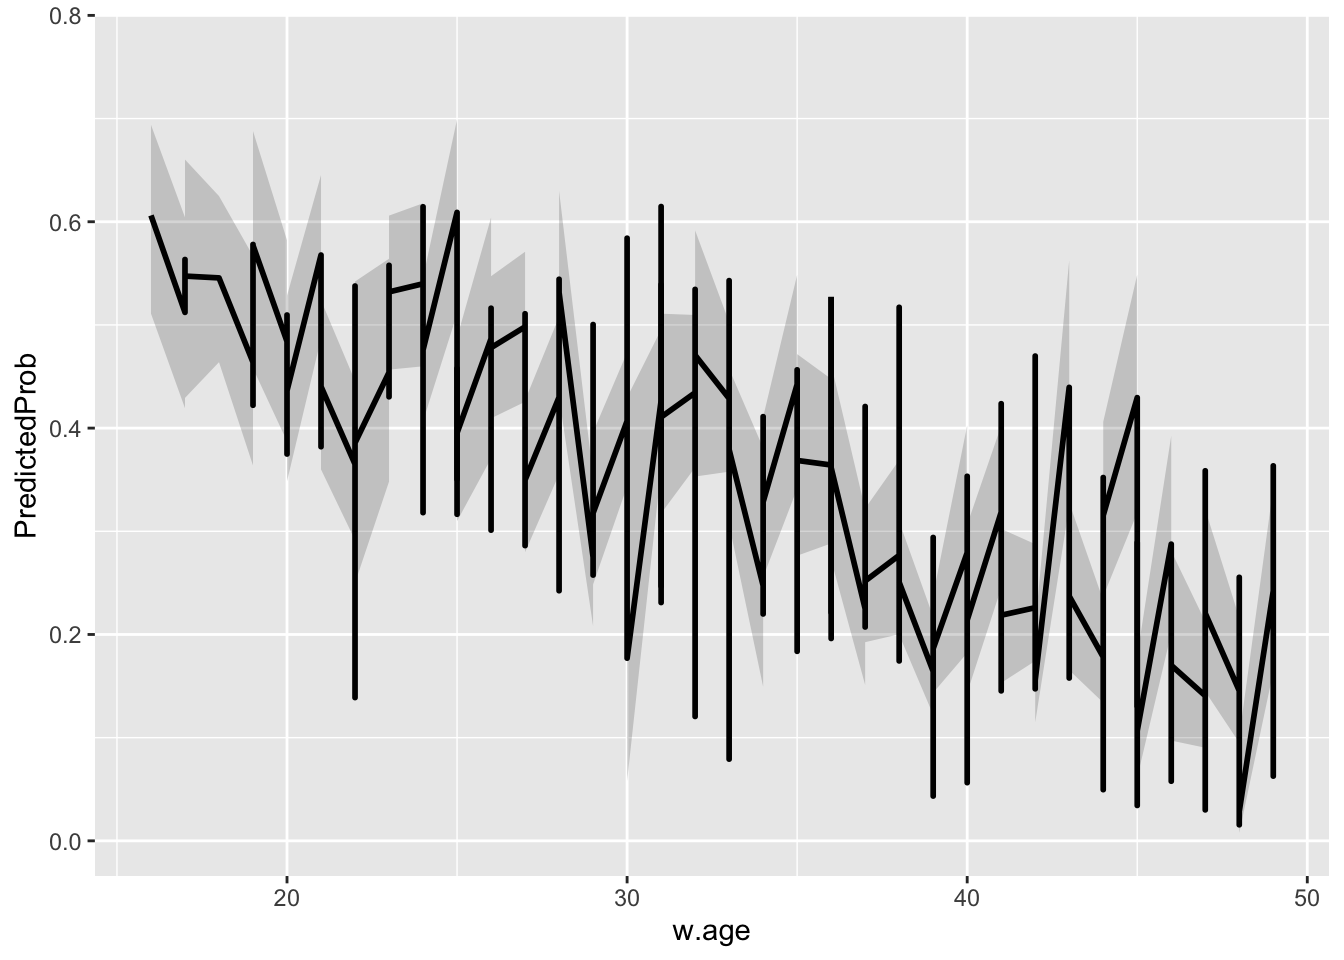
\includegraphics{rule-mining_files/figure-latex/unnamed-chunk-14-1} \end{center}

The scatter plot gives us information about how support-confidence-lift
measures are distributed along retained rules. However, it is not very
helpful to actually see which rules have which values.

To see the relationship between rules we can use either a balloon plot
or parallel coordinates graph.

\hypertarget{balloon-plot}{%
\subsubsection{Balloon Plot}\label{balloon-plot}}

\begin{Shaded}
\begin{Highlighting}[]
\KeywordTok{plot}\NormalTok{(rules.pruned, }\DataTypeTok{method=}\StringTok{"graph"}\NormalTok{, }\DataTypeTok{control=}\KeywordTok{list}\NormalTok{(}\DataTypeTok{type=}\StringTok{"items"}\NormalTok{))}
\end{Highlighting}
\end{Shaded}

\begin{verbatim}
## Available control parameters (with default values):
## main  =  Graph for 8 rules
## nodeColors    =  c("#66CC6680", "#9999CC80")
## nodeCol   =  c("#EE0000FF", "#EE0303FF", "#EE0606FF", "#EE0909FF", "#EE0C0CFF", "#EE0F0FFF", "#EE1212FF", "#EE1515FF", "#EE1818FF", "#EE1B1BFF", "#EE1E1EFF", "#EE2222FF", "#EE2525FF", "#EE2828FF", "#EE2B2BFF", "#EE2E2EFF", "#EE3131FF", "#EE3434FF", "#EE3737FF", "#EE3A3AFF", "#EE3D3DFF", "#EE4040FF", "#EE4444FF", "#EE4747FF", "#EE4A4AFF", "#EE4D4DFF", "#EE5050FF", "#EE5353FF", "#EE5656FF", "#EE5959FF", "#EE5C5CFF", "#EE5F5FFF", "#EE6262FF", "#EE6666FF", "#EE6969FF", "#EE6C6CFF", "#EE6F6FFF", "#EE7272FF", "#EE7575FF",  "#EE7878FF", "#EE7B7BFF", "#EE7E7EFF", "#EE8181FF", "#EE8484FF", "#EE8888FF", "#EE8B8BFF", "#EE8E8EFF", "#EE9191FF", "#EE9494FF", "#EE9797FF", "#EE9999FF", "#EE9B9BFF", "#EE9D9DFF", "#EE9F9FFF", "#EEA0A0FF", "#EEA2A2FF", "#EEA4A4FF", "#EEA5A5FF", "#EEA7A7FF", "#EEA9A9FF", "#EEABABFF", "#EEACACFF", "#EEAEAEFF", "#EEB0B0FF", "#EEB1B1FF", "#EEB3B3FF", "#EEB5B5FF", "#EEB7B7FF", "#EEB8B8FF", "#EEBABAFF", "#EEBCBCFF", "#EEBDBDFF", "#EEBFBFFF", "#EEC1C1FF", "#EEC3C3FF", "#EEC4C4FF", "#EEC6C6FF", "#EEC8C8FF",  "#EEC9C9FF", "#EECBCBFF", "#EECDCDFF", "#EECFCFFF", "#EED0D0FF", "#EED2D2FF", "#EED4D4FF", "#EED5D5FF", "#EED7D7FF", "#EED9D9FF", "#EEDBDBFF", "#EEDCDCFF", "#EEDEDEFF", "#EEE0E0FF", "#EEE1E1FF", "#EEE3E3FF", "#EEE5E5FF", "#EEE7E7FF", "#EEE8E8FF", "#EEEAEAFF", "#EEECECFF", "#EEEEEEFF")
## edgeCol   =  c("#474747FF", "#494949FF", "#4B4B4BFF", "#4D4D4DFF", "#4F4F4FFF", "#515151FF", "#535353FF", "#555555FF", "#575757FF", "#595959FF", "#5B5B5BFF", "#5E5E5EFF", "#606060FF", "#626262FF", "#646464FF", "#666666FF", "#686868FF", "#6A6A6AFF", "#6C6C6CFF", "#6E6E6EFF", "#707070FF", "#727272FF", "#747474FF", "#767676FF", "#787878FF", "#7A7A7AFF", "#7C7C7CFF", "#7E7E7EFF", "#808080FF", "#828282FF", "#848484FF", "#868686FF", "#888888FF", "#8A8A8AFF", "#8C8C8CFF", "#8D8D8DFF", "#8F8F8FFF", "#919191FF", "#939393FF",  "#959595FF", "#979797FF", "#999999FF", "#9A9A9AFF", "#9C9C9CFF", "#9E9E9EFF", "#A0A0A0FF", "#A2A2A2FF", "#A3A3A3FF", "#A5A5A5FF", "#A7A7A7FF", "#A9A9A9FF", "#AAAAAAFF", "#ACACACFF", "#AEAEAEFF", "#AFAFAFFF", "#B1B1B1FF", "#B3B3B3FF", "#B4B4B4FF", "#B6B6B6FF", "#B7B7B7FF", "#B9B9B9FF", "#BBBBBBFF", "#BCBCBCFF", "#BEBEBEFF", "#BFBFBFFF", "#C1C1C1FF", "#C2C2C2FF", "#C3C3C4FF", "#C5C5C5FF", "#C6C6C6FF", "#C8C8C8FF", "#C9C9C9FF", "#CACACAFF", "#CCCCCCFF", "#CDCDCDFF", "#CECECEFF", "#CFCFCFFF", "#D1D1D1FF",  "#D2D2D2FF", "#D3D3D3FF", "#D4D4D4FF", "#D5D5D5FF", "#D6D6D6FF", "#D7D7D7FF", "#D8D8D8FF", "#D9D9D9FF", "#DADADAFF", "#DBDBDBFF", "#DCDCDCFF", "#DDDDDDFF", "#DEDEDEFF", "#DEDEDEFF", "#DFDFDFFF", "#E0E0E0FF", "#E0E0E0FF", "#E1E1E1FF", "#E1E1E1FF", "#E2E2E2FF", "#E2E2E2FF", "#E2E2E2FF")
## alpha     =  0.5
## cex   =  1
## itemLabels    =  TRUE
## labelCol  =  #000000B3
## measureLabels     =  FALSE
## precision     =  3
## layout    =  NULL
## layoutParams  =  list()
## arrowSize     =  0.5
## engine    =  igraph
## plot  =  TRUE
## plot_options  =  list()
## max   =  100
## verbose   =  FALSE
\end{verbatim}

\begin{center}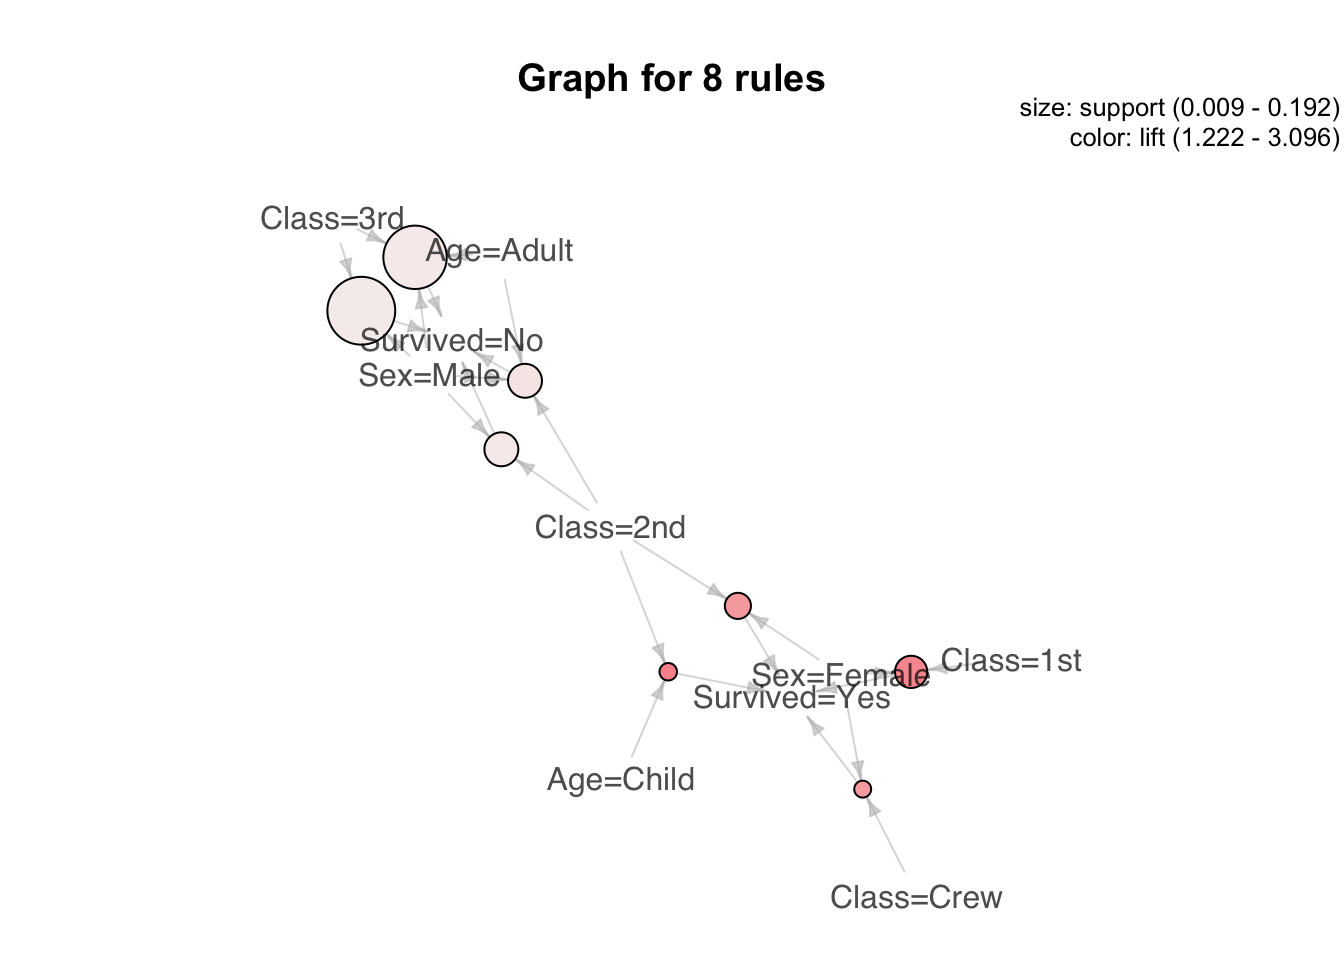
\includegraphics{rule-mining_files/figure-latex/unnamed-chunk-15-1} \end{center}

The balloon plot gives us information about the rules, support and lift
measures. However it doesn't give us any information about confidence
levels.

\hypertarget{parallel-coordinates-plot}{%
\subsubsection{Parallel Coordinates
Plot}\label{parallel-coordinates-plot}}

\begin{Shaded}
\begin{Highlighting}[]
\KeywordTok{plot}\NormalTok{(rules.pruned, }\DataTypeTok{method=}\StringTok{"paracoord"}\NormalTok{, }\DataTypeTok{control=}\KeywordTok{list}\NormalTok{(}\DataTypeTok{reorder=}\OtherTok{TRUE}\NormalTok{))}
\end{Highlighting}
\end{Shaded}

\begin{center}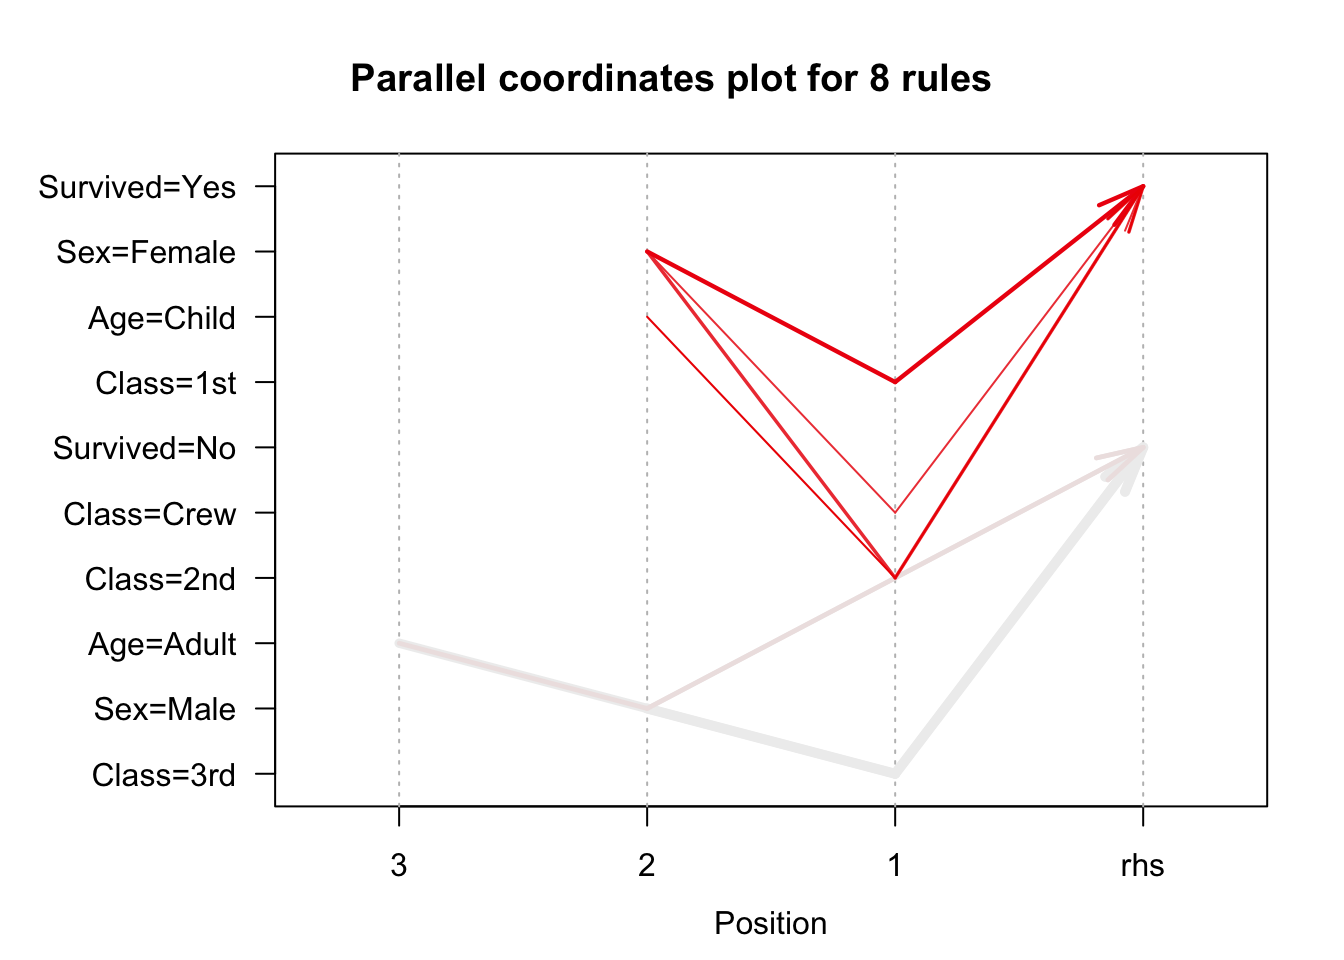
\includegraphics{rule-mining_files/figure-latex/unnamed-chunk-16-1} \end{center}

Parallel coordinates plots give us an excellent picture of rules.

\hypertarget{useful-links}{%
\subsection{Useful Links}\label{useful-links}}

\begin{itemize}
\tightlist
\item
  Association Mining datasets: \url{http://fimi.ua.ac.be/data/}

  \begin{itemize}
  \tightlist
  \item
    This webpage holds datasets for association mining
  \end{itemize}
\item
  Information about sequential association mining techniques:
  \url{http://research.microsoft.com/pubs/217091/gupta11a_apdsdm.pdf}

  \begin{itemize}
  \tightlist
  \item
    This document holds information regarding a somewhat more advanced
    topic: sequential mining
  \end{itemize}
\item
  Mining frequent items bought together using Apriori Algorithm:
  \url{https://www.analyticsvidhya.com/blog/2017/08/mining-frequent-items-using-apriori-algorithm/}
\end{itemize}

\end{document}
